\section{Systematic uncertainties}
\label{sec:systematics}

This section describes the main sources of systematic uncertainty considered.
Other sources, which would matter in measurements of absolute quantities,
cancel in the ratio between the rare and resonant channels.
The systematic uncertainties considered and their estimated effects on the \RKst
ratio are summarised in Tab.~\ref{tab:systematics}; more details about each source are 
given in the following sections. The total uncertainty is evaluated by summing in quadrature 
the individual components and results in $\sim  2\%$ for the low- and central-\qsq intervals
and $\sim  9\%$ for the high-\qsq interval. 
%These studies are preliminary.
This evaluation of systematic uncertainties represents the current status of 
the analysis at the time of writing, and may evolve prior to publication.

\vspace{0.5cm}

\begin{table}[h!]
\begin{center}
\caption{Summary of the systematic uncertainties on the \RKst ratio (\%).}
\renewcommand\arraystretch{1.25}
\label{tab:systematics}
\begin{tabular}{$c|^c|^c|^c}
\rowstyle{\bfseries}
\textbf{Source} & low-\boldmath{\qsq} (\%) & central-\boldmath{\qsq} (\%) & high-\boldmath{\qsq} (\%)\\ \hline

Signal shape		    	 & 1.65      & 1.10      & 2.92 \\
Bremsstrahlung categories & 0.04  & 0.06  & 0.37 \\
%Trigger categories	    &        & 	      &  \\

\hline

Swap			        & 0.30        & 0.12	      & 0.13 \\
$\Lb\to pK\ll$ 		    	& 0.25             & 0.28	      & 0.77 \\
%\BsToKstJPsll		    &           & 	      &  \\

%Partially-reconstructed	    & 0.11     & 4.13     & 0.10 \\
%\LbTopKll       		    &          & 	      &  \\
Combinatorial 		    	& 0.00        & 0.02	      & 8.02 \\

%\BdToKstGee leakage    &       &       &  \\
\jpsi leakage    			& 0.06      & 0.01      & 0.10 \\
\psitwos leakage    		& 0.03      & 0.01      & 2.00 \\
PDF smoothing   		& 0.11       & 0.28      & 0.49 \\

%\verb!RooKeysPdf! ($\rho=1.1$)    & 0.11       & 0.28      & 0.14 \\
%\verb!RooKeysPdf! ($\rho=1.3$)    & 0.10       & 0.24      & 0.49 \\

\hline

Efficiency		        & 0.65          & 0.74	      & 0.83 \\
%TISTOS			& 2.47	& 2.30	& 2.80 \\
Bin migration               & 0.69                & 1.43                      & 1.19    \\


%\hline

%Total				& 	      &  \\

\end{tabular}
\end{center}
\end{table}


\subsection{Choice of signal and background PDFs}

There is a certain arbitrariness in the choice of PDFs used to model signal and background contributions in the
invariant mass fits, which could translate into a bias on the final result. The systematic uncertainty due to the
parameterisation of the line shapes is studied in the following ways.

For the signal PDF:
%
\begin{itemize}

\item \textit{Shape}: in the electron channels the PDF is changed from a CBG to a DCB function.
Modifying the PDF has a negligible effect in the muon modes, while it affects the electron ones.
 Furthermore the data-simulation discrepancy parameters ($m'$ and $c$) are constrained using the
\BdToKstGee sample instead of \BdToKstJPsee.

\item \textit{Bremsstrahlung categories}: Gaussian constraints are applied to the relative fractions of 
the bremsstrahlung categories, instead of fixing them to the values observed on simulation.
%This yields a $\sim \%$ systematic on \RKst in the central- and high-\qsq region.

%\item \textit{Trigger categories}: the fit is repeated without splitting the electron sample in trigger categories;
%this results in a $\sim \%$ ($\sim \%$) variation on \RKst in the central-\qsq (high-\qsq) region;

\end{itemize}

For the background PDFs:
%
\begin{itemize}

\item \textit{Swaps}: a component that describes candidates where the particle identities are swapped
is added both to the muon and electron resonant fits, and constrained to the number of candidates
expected from simulation. 
%This amounts to a $\sim \%$ variation on \RKst in the central- and high-\qsq region.

%\item $\Lb\to pK\jpsi(\to \ee)$: the normalisation is left free to vary.
%This results in a $\sim \%$ variation on \RKst in the central- and high-\qsq region.

%\item $\Bs\to\Kstarz\jpsi(\to \ll)$: the $\Bs\to\Kstarz\jpsi(\to \mumu)$ shape is taken from simulation
%instead of using the same shape as for the signal. The normalisation is fixed
%to the branching ratio times the production fraction.
%This results in a $\sim \%$ variation on \RKst in the central- and high-\qsq region.

%\item \textit{Partially-reconstructed}: the yield of the mis-reconstructed background to \BdToKstee is left free to vary in the fit.
%This only applies to the central-\qsq interval as this contribution is already free to vary in the high-\qsq range.
%This yields a $\sim \%$ systematic on \RKst.

\item \textit{Combinatorial}: the PDF is changed from an exponential to the shape of a background-enriched sample, obtained using 
an anti-MVA requirement; the opposite is done for the high-\qsq interval, where the anti-MVA shape is the nominal one. 
%This amounts to a $\sim \%$ variation on \RKst in the central- and high-\qsq region.

\item $\Lb\to pK \ll$: this background is added to the fit for the rare channel and returns zero yield for both the muon 
and the electron samples. Therefore, no systematic uncertainty is assigned from this source. Furthermore, the $\Lb\to pK\jpsi(\to \ee)$ 
normalisation is allowed to vary on the fit rather than being fixed to the value predicted using the \Lb yield in the muon channel.

\item \textit{Leakage}: the amounts of the leakages, which are fixed in the nominal fit to the corresponding signal yields, are allowed to vary.
%This results in a $\sim \%$ variation on \RKst in the central- and high-\qsq region.

\item \textit{PDF smoothing}: in all cases where a simulated sample is used to obtain background shapes and smoothed to obtain a PDF,
the kernel of the density estimation is varied by $\pm\, 0.1$ from the value used in the nominal fit.
The largest difference from the default values is assigned as a systematic uncertainty.

\end{itemize}

\subsection{Efficiency determination}

The statistical uncertainty on the efficiency determination due to the finite size of the simulated 
and calibration samples is taken as the corresponding systematic uncertainty.
%The correlation among the electron trigger categories is taken into account (e.g. L0E and L0H are anti-correlated).
%This amounts to a $\sim \%$ ($\sim \%$) systematic uncertainty on \RKst for the central-\qsq (high-\qsq) interval.
%
A further source of systematic uncertainty associated with the trigger efficiency is estimated using the data-simulation
differences observed in Sec.~\ref{sec:tistos}. Ratios of efficiencies for the rare to resonant decays are found to be 
compatible between the electron and muon modes, indicating that the effect on \RKst is negligible, 
therefore no uncertainty is assigned for this source.
%, but the statistical precision on the determinations is taken as an extra systematic uncertainty.

%A further source of systematic, which is considered, is due to the
%discrepancies found in Sec.~\ref{sec:tistos} on the determination of the trigger efficiency. 
%As explained in that subsection the efficiency is derived as a function of the relevant
%kinematic quantities for each trigger category. The efficiency
%is then obtained for the rare and resonant sample by a weighted average.
%These are found to be compatible indicating that the effect on the
%ratios between rare and resonant channels is negligible.
%Therefore, no systematic uncertainty is added for this source.

\subsection{Bin migration}

The determination of the reconstruction efficiency is affected by the knowledge of the
amount of bin migration as explained in Sec.~\ref{sec:reco_binmig}. This amount depends
on the shape of the \qsq distribution, which in turn depends on the simulated \mbox{\BdToKstee} decay model.
In order to assess this systematic, simulated samples are generated using different
models corresponding to different form factors~\cite{Ball:2004ye,Aoki:2013ldr,Melikhov:2000yu}.
The \qsq distributions obtained using each model are compared with those obtained using
the default model~\cite{Ali:1999mm}.
Figure~\ref{fig:q2ratios} shows the ratios of these \qsq distributions relative to the default model, 
which are used to re-weight the simulation. The amount of bin migration is calculated
using the simulation re-weighted to reproduce each model; Table~\ref{tab:sys_binmig} lists the
percent variations obtained. The largest difference between two values is taken as systematic uncertainty.
%This results in a $\sim5\%$ uncertainty for the central-\qsq interval and $\sim11\%$ for the high-\qsq one,
%which represent in both channel the biggest systematic uncertainty.
\begin{table}[h!]
\centering
\caption{Variation on the level of bin migration (\%) obtained using different form factors models.}
\begin{tabular}{$c|^c^c^c}
\rowstyle{\bfseries}
Model                   		& low-\boldmath{\qsq} & central-\boldmath{\qsq}  &  central-\boldmath{\qsq} \\ \hline
Ball-Zwicky~\cite{Ball:2004ye}         		& -0.3          & 1.0          & 0.2 \\
%%Melikhov Stech  					& 4.8          & -3.2          & 6.8 \\
Colangelo~\cite{Aoki:2013ldr}			& 0.4          & 0.4 	        & 0.8 \\
Melikhov lattice~\cite{Melikhov:2000yu}    & 0.1          & -0.4          & -0.4 \\
\end{tabular}
\label{tab:sys_binmig}
\end{table}
%
\begin{figure}[h!]
\centering 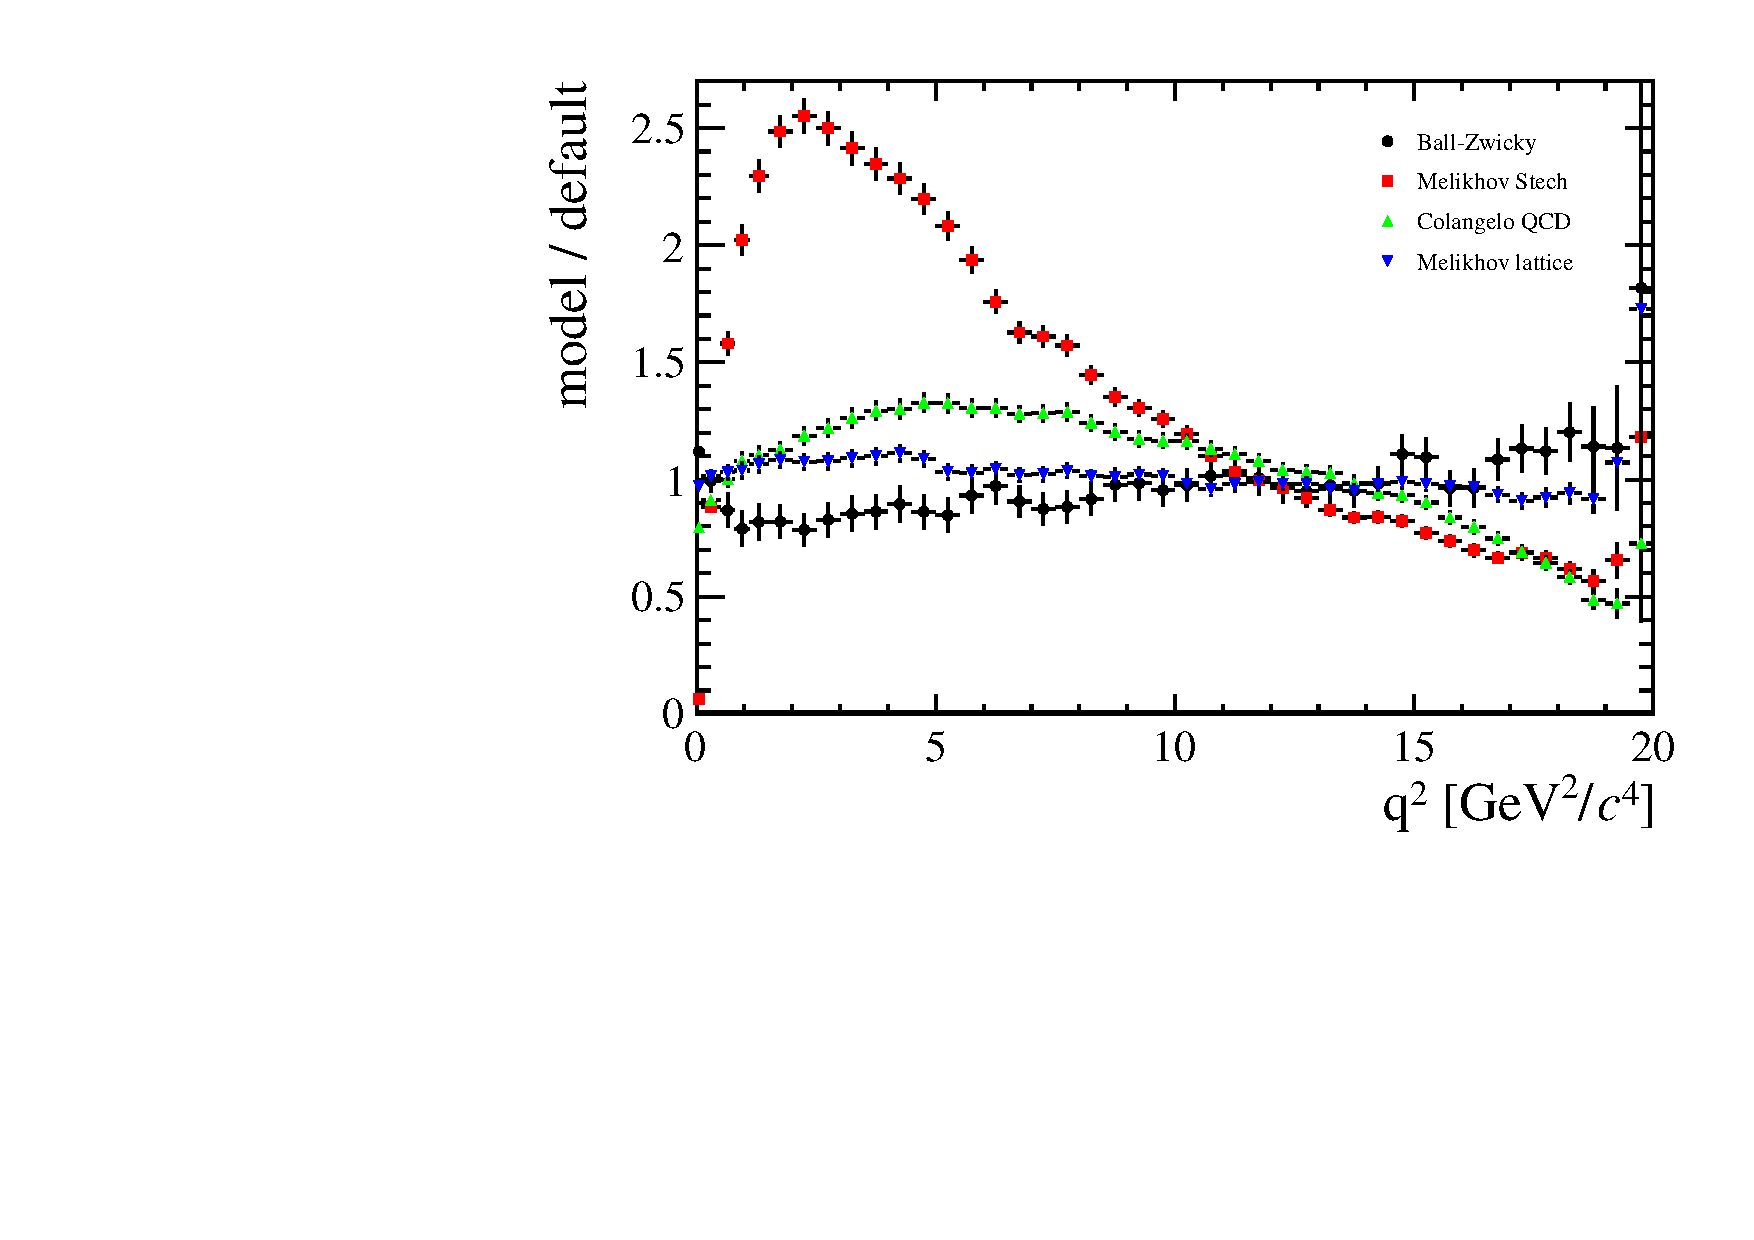
\includegraphics[width=0.8\textwidth]{RKst/figs/models_ratios.pdf}
\caption{Ratios of the \qsq distributions obtained using different form
factors models~\cite{Ball:2004ye,Aoki:2013ldr,Melikhov:2000yu} with respect 
to the default model~\cite{Ali:1999mm}. }
\label{fig:q2ratios}
\end{figure}
%




